%********************************************%
%*       Generated from PreTeXt source      *%
%*       on 2022-04-19T13:43:00-04:00       *%
%*   A recent stable commit (2020-08-09):   *%
%* 98f21740783f166a773df4dc83cab5293ab63a4a *%
%*                                          *%
%*         https://pretextbook.org          *%
%*                                          *%
%********************************************%
%% We elect to always write snapshot output into <job>.dep file
\RequirePackage{snapshot}
\documentclass[twoside,10pt,]{book}
%% Custom Preamble Entries, early (use latex.preamble.early)
%% Default LaTeX packages
%%   1.  always employed (or nearly so) for some purpose, or
%%   2.  a stylewriter may assume their presence
\usepackage{geometry}
%% Some aspects of the preamble are conditional,
%% the LaTeX engine is one such determinant
\usepackage{ifthen}
%% etoolbox has a variety of modern conveniences
\usepackage{etoolbox}
\usepackage{ifxetex,ifluatex}
%% Raster graphics inclusion
\usepackage{graphicx}
%% Color support, xcolor package
%% Always loaded, for: add/delete text, author tools
%% Here, since tcolorbox loads tikz, and tikz loads xcolor
\PassOptionsToPackage{usenames,dvipsnames,svgnames,table}{xcolor}
\usepackage{xcolor}
%% begin: defined colors, via xcolor package, for styling
%% end: defined colors, via xcolor package, for styling
%% Colored boxes, and much more, though mostly styling
%% skins library provides "enhanced" skin, employing tikzpicture
%% boxes may be configured as "breakable" or "unbreakable"
%% "raster" controls grids of boxes, aka side-by-side
\usepackage{tcolorbox}
\tcbuselibrary{skins}
\tcbuselibrary{breakable}
\tcbuselibrary{raster}
%% We load some "stock" tcolorbox styles that we use a lot
%% Placement here is provisional, there will be some color work also
%% First, black on white, no border, transparent, but no assumption about titles
\tcbset{ bwminimalstyle/.style={size=minimal, boxrule=-0.3pt, frame empty,
colback=white, colbacktitle=white, coltitle=black, opacityfill=0.0} }
%% Second, bold title, run-in to text/paragraph/heading
%% Space afterwards will be controlled by environment,
%% independent of constructions of the tcb title
%% Places \blocktitlefont onto many block titles
\tcbset{ runintitlestyle/.style={fonttitle=\blocktitlefont\upshape\bfseries, attach title to upper} }
%% Spacing prior to each exercise, anywhere
\tcbset{ exercisespacingstyle/.style={before skip={1.5ex plus 0.5ex}} }
%% Spacing prior to each block
\tcbset{ blockspacingstyle/.style={before skip={2.0ex plus 0.5ex}} }
%% xparse allows the construction of more robust commands,
%% this is a necessity for isolating styling and behavior
%% The tcolorbox library of the same name loads the base library
\tcbuselibrary{xparse}
%% The tcolorbox library loads TikZ, its calc package is generally useful,
%% and is necessary for some smaller documents that use partial tcolor boxes
%% See:  https://github.com/PreTeXtBook/pretext/issues/1624
\usetikzlibrary{calc}
%% Hyperref should be here, but likes to be loaded late
%%
%% Inline math delimiters, \(, \), need to be robust
%% 2016-01-31:  latexrelease.sty  supersedes  fixltx2e.sty
%% If  latexrelease.sty  exists, bugfix is in kernel
%% If not, bugfix is in  fixltx2e.sty
%% See:  https://tug.org/TUGboat/tb36-3/tb114ltnews22.pdf
%% and read "Fewer fragile commands" in distribution's  latexchanges.pdf
\IfFileExists{latexrelease.sty}{}{\usepackage{fixltx2e}}
%% Footnote counters and part/chapter counters are manipulated
%% April 2018:  chngcntr  commands now integrated into the kernel,
%% but circa 2018/2019 the package would still try to redefine them,
%% so we need to do the work of loading conditionally for old kernels.
%% From version 1.1a,  chngcntr  should detect defintions made by LaTeX kernel.
\ifdefined\counterwithin
\else
    \usepackage{chngcntr}
\fi
%% Text height identically 9 inches, text width varies on point size
%% See Bringhurst 2.1.1 on measure for recommendations
%% 75 characters per line (count spaces, punctuation) is target
%% which is the upper limit of Bringhurst's recommendations
\geometry{letterpaper,total={340pt,9.0in}}
%% Custom Page Layout Adjustments (use latex.geometry)
%% This LaTeX file may be compiled with pdflatex, xelatex, or lualatex executables
%% LuaTeX is not explicitly supported, but we do accept additions from knowledgeable users
%% The conditional below provides  pdflatex  specific configuration last
%% begin: engine-specific capabilities
\ifthenelse{\boolean{xetex} \or \boolean{luatex}}{%
%% begin: xelatex and lualatex-specific default configuration
\ifxetex\usepackage{xltxtra}\fi
%% realscripts is the only part of xltxtra relevant to lualatex 
\ifluatex\usepackage{realscripts}\fi
%% end:   xelatex and lualatex-specific default configuration
}{
%% begin: pdflatex-specific default configuration
%% We assume a PreTeXt XML source file may have Unicode characters
%% and so we ask LaTeX to parse a UTF-8 encoded file
%% This may work well for accented characters in Western language,
%% but not with Greek, Asian languages, etc.
%% When this is not good enough, switch to the  xelatex  engine
%% where Unicode is better supported (encouraged, even)
\usepackage[utf8]{inputenc}
%% end: pdflatex-specific default configuration
}
%% end:   engine-specific capabilities
%%
%% Fonts.  Conditional on LaTex engine employed.
%% Default Text Font: The Latin Modern fonts are
%% "enhanced versions of the [original TeX] Computer Modern fonts."
%% We use them as the default text font for PreTeXt output.
%% Default Monospace font: Inconsolata (aka zi4)
%% Sponsored by TUG: http://levien.com/type/myfonts/inconsolata.html
%% Loaded for documents with intentional objects requiring monospace
%% See package documentation for excellent instructions
%% fontspec will work universally if we use filename to locate OTF files
%% Loads the "upquote" package as needed, so we don't have to
%% Upright quotes might come from the  textcomp  package, which we also use
%% We employ the shapely \ell to match Google Font version
%% pdflatex: "varl" package option produces shapely \ell
%% pdflatex: "var0" package option produces plain zero (not used)
%% pdflatex: "varqu" package option produces best upright quotes
%% xelatex,lualatex: add OTF StylisticSet 1 for shapely \ell
%% xelatex,lualatex: add OTF StylisticSet 2 for plain zero (not used)
%% xelatex,lualatex: add OTF StylisticSet 3 for upright quotes
%%
%% Automatic Font Control
%% Portions of a document, are, or may, be affected by defined commands
%% These are perhaps more flexible when using  xelatex  rather than  pdflatex
%% The following definitions are meant to be re-defined in a style, using \renewcommand
%% They are scoped when employed (in a TeX group), and so should not be defined with an argument
\newcommand{\divisionfont}{\relax}
\newcommand{\blocktitlefont}{\relax}
\newcommand{\contentsfont}{\relax}
\newcommand{\pagefont}{\relax}
\newcommand{\tabularfont}{\relax}
\newcommand{\xreffont}{\relax}
\newcommand{\titlepagefont}{\relax}
%%
\ifthenelse{\boolean{xetex} \or \boolean{luatex}}{%
%% begin: font setup and configuration for use with xelatex
%% Generally, xelatex is necessary for non-Western fonts
%% fontspec package provides extensive control of system fonts,
%% meaning *.otf (OpenType), and apparently *.ttf (TrueType)
%% that live *outside* your TeX/MF tree, and are controlled by your *system*
%% (it is possible that a TeX distribution will place fonts in a system location)
%%
%% The fontspec package is the best vehicle for using different fonts in  xelatex
%% So we load it always, no matter what a publisher or style might want
%%
\usepackage{fontspec}
%%
%% begin: xelatex main font ("font-xelatex-main" template)
%% Latin Modern Roman is the default font for xelatex and so is loaded with a TU encoding
%% *in the format* so we can't touch it, only perhaps adjust it later
%% in one of two ways (then known by NFSS names such as "lmr")
%% (1) via NFSS with font family names such as "lmr" and "lmss"
%% (2) via fontspec with commands like \setmainfont{Latin Modern Roman}
%% The latter requires the font to be known at the system-level by its font name,
%% but will give access to OTF font features through optional arguments
%% https://tex.stackexchange.com/questions/470008/
%% where-and-how-does-fontspec-sty-specify-the-default-font-latin-modern-roman
%% http://tex.stackexchange.com/questions/115321
%% /how-to-optimize-latin-modern-font-with-xelatex
%%
%% end:   xelatex main font ("font-xelatex-main" template)
%% begin: xelatex mono font ("font-xelatex-mono" template)
%% (conditional on non-trivial uses being present in source)
\IfFontExistsTF{Inconsolatazi4-Regular.otf}{}{\GenericError{}{The font "Inconsolatazi4-Regular.otf" requested by PreTeXt output is not available.  Either a file cannot be located in default locations via a filename, or a font is not known by its name as part of your system.}{Consult the PreTeXt Guide for help with LaTeX fonts.}{}}
\IfFontExistsTF{Inconsolatazi4-Bold.otf}{}{\GenericError{}{The font "Inconsolatazi4-Bold.otf" requested by PreTeXt output is not available.  Either a file cannot be located in default locations via a filename, or a font is not known by its name as part of your system.}{Consult the PreTeXt Guide for help with LaTeX fonts.}{}}
\usepackage{zi4}
\setmonofont[BoldFont=Inconsolatazi4-Bold.otf,StylisticSet={1,3}]{Inconsolatazi4-Regular.otf}
%% end:   xelatex mono font ("font-xelatex-mono" template)
%% begin: xelatex font adjustments ("font-xelatex-style" template)
%% end:   xelatex font adjustments ("font-xelatex-style" template)
%%
%% Extensive support for other languages
\usepackage{polyglossia}
%% Set main/default language based on pretext/@xml:lang value
%% document language code is "en-US", US English
%% usmax variant has extra hypenation
\setmainlanguage[variant=usmax]{english}
%% Enable secondary languages based on discovery of @xml:lang values
%% Enable fonts/scripts based on discovery of @xml:lang values
%% Western languages should be ably covered by Latin Modern Roman
%% end:   font setup and configuration for use with xelatex
}{%
%% begin: font setup and configuration for use with pdflatex
%% begin: pdflatex main font ("font-pdflatex-main" template)
\usepackage{lmodern}
\usepackage[T1]{fontenc}
%% end:   pdflatex main font ("font-pdflatex-main" template)
%% begin: pdflatex mono font ("font-pdflatex-mono" template)
%% (conditional on non-trivial uses being present in source)
\usepackage[varqu,varl]{inconsolata}
%% end:   pdflatex mono font ("font-pdflatex-mono" template)
%% begin: pdflatex font adjustments ("font-pdflatex-style" template)
%% end:   pdflatex font adjustments ("font-pdflatex-style" template)
%% end:   font setup and configuration for use with pdflatex
}
%% Micromanage spacing, etc.  The named "microtype-options"
%% template may be employed to fine-tune package behavior
\usepackage{microtype}
%% Symbols, align environment, commutative diagrams, bracket-matrix
\usepackage{amsmath}
\usepackage{amscd}
\usepackage{amssymb}
%% allow page breaks within display mathematics anywhere
%% level 4 is maximally permissive
%% this is exactly the opposite of AMSmath package philosophy
%% there are per-display, and per-equation options to control this
%% split, aligned, gathered, and alignedat are not affected
\allowdisplaybreaks[4]
%% allow more columns to a matrix
%% can make this even bigger by overriding with  latex.preamble.late  processing option
\setcounter{MaxMatrixCols}{30}
%%
%%
%% Division Titles, and Page Headers/Footers
%% titlesec package, loading "titleps" package cooperatively
%% See code comments about the necessity and purpose of "explicit" option.
%% The "newparttoc" option causes a consistent entry for parts in the ToC 
%% file, but it is only effective if there is a \titleformat for \part.
%% "pagestyles" loads the  titleps  package cooperatively.
\usepackage[explicit, newparttoc, pagestyles]{titlesec}
%% The companion titletoc package for the ToC.
\usepackage{titletoc}
%% Fixes a bug with transition from chapters to appendices in a "book"
%% See generating XSL code for more details about necessity
\newtitlemark{\chaptertitlename}
%% begin: customizations of page styles via the modal "titleps-style" template
%% Designed to use commands from the LaTeX "titleps" package
%% Plain pages should have the same font for page numbers
\renewpagestyle{plain}{%
\setfoot{}{\pagefont\thepage}{}%
}%
%% Two-page spread as in default LaTeX
\renewpagestyle{headings}{%
\sethead%
[\pagefont\thepage]%
[]
[\pagefont\slshape\MakeUppercase{\ifthechapter{\chaptertitlename\space\thechapter.\space}{}\chaptertitle}]%
{\pagefont\slshape\MakeUppercase{\ifthesection{Section\space\thesection.\space\sectiontitle}{}}}%
{}%
{\pagefont\thepage}%
}%
\pagestyle{headings}
%% end: customizations of page styles via the modal "titleps-style" template
%%
%% Create globally-available macros to be provided for style writers
%% These are redefined for each occurence of each division
\newcommand{\divisionnameptx}{\relax}%
\newcommand{\titleptx}{\relax}%
\newcommand{\subtitleptx}{\relax}%
\newcommand{\shortitleptx}{\relax}%
\newcommand{\authorsptx}{\relax}%
\newcommand{\epigraphptx}{\relax}%
%% Create environments for possible occurences of each division
%% Environment for a PTX "acknowledgement" at the level of a LaTeX "chapter"
\NewDocumentEnvironment{acknowledgement}{mmmmmm}
{%
\renewcommand{\divisionnameptx}{Acknowledgements}%
\renewcommand{\titleptx}{#1}%
\renewcommand{\subtitleptx}{#2}%
\renewcommand{\shortitleptx}{#3}%
\renewcommand{\authorsptx}{#4}%
\renewcommand{\epigraphptx}{#5}%
\chapter*{#1}%
\addcontentsline{toc}{chapter}{#3}
\label{#6}%
}{}%
%% Environment for a PTX "preface" at the level of a LaTeX "chapter"
\NewDocumentEnvironment{preface}{mmmmmm}
{%
\renewcommand{\divisionnameptx}{Preface}%
\renewcommand{\titleptx}{#1}%
\renewcommand{\subtitleptx}{#2}%
\renewcommand{\shortitleptx}{#3}%
\renewcommand{\authorsptx}{#4}%
\renewcommand{\epigraphptx}{#5}%
\chapter*{#1}%
\addcontentsline{toc}{chapter}{#3}
\label{#6}%
}{}%
%% Environment for a PTX "chapter" at the level of a LaTeX "chapter"
\NewDocumentEnvironment{chapterptx}{mmmmmm}
{%
\renewcommand{\divisionnameptx}{Chapter}%
\renewcommand{\titleptx}{#1}%
\renewcommand{\subtitleptx}{#2}%
\renewcommand{\shortitleptx}{#3}%
\renewcommand{\authorsptx}{#4}%
\renewcommand{\epigraphptx}{#5}%
\chapter[{#3}]{#1}%
\label{#6}%
}{}%
%% Environment for a PTX "section" at the level of a LaTeX "section"
\NewDocumentEnvironment{sectionptx}{mmmmmm}
{%
\renewcommand{\divisionnameptx}{Section}%
\renewcommand{\titleptx}{#1}%
\renewcommand{\subtitleptx}{#2}%
\renewcommand{\shortitleptx}{#3}%
\renewcommand{\authorsptx}{#4}%
\renewcommand{\epigraphptx}{#5}%
\section[{#3}]{#1}%
\label{#6}%
}{}%
%% Environment for a PTX "subsection" at the level of a LaTeX "subsection"
\NewDocumentEnvironment{subsectionptx}{mmmmmm}
{%
\renewcommand{\divisionnameptx}{Subsection}%
\renewcommand{\titleptx}{#1}%
\renewcommand{\subtitleptx}{#2}%
\renewcommand{\shortitleptx}{#3}%
\renewcommand{\authorsptx}{#4}%
\renewcommand{\epigraphptx}{#5}%
\subsection[{#3}]{#1}%
\label{#6}%
}{}%
%% Environment for a PTX "worksheet" at the level of a LaTeX "subsection"
\NewDocumentEnvironment{worksheet-subsection}{mmmmmm}
{%
\renewcommand{\divisionnameptx}{Worksheet}%
\renewcommand{\titleptx}{#1}%
\renewcommand{\subtitleptx}{#2}%
\renewcommand{\shortitleptx}{#3}%
\renewcommand{\authorsptx}{#4}%
\renewcommand{\epigraphptx}{#5}%
\subsection[{#3}]{#1}%
\label{#6}%
}{}%
%% Environment for a PTX "worksheet" at the level of a LaTeX "subsection"
\NewDocumentEnvironment{worksheet-subsection-numberless}{mmmmmm}
{%
\renewcommand{\divisionnameptx}{Worksheet}%
\renewcommand{\titleptx}{#1}%
\renewcommand{\subtitleptx}{#2}%
\renewcommand{\shortitleptx}{#3}%
\renewcommand{\authorsptx}{#4}%
\renewcommand{\epigraphptx}{#5}%
\subsection*{#1}%
\addcontentsline{toc}{subsection}{#3}
\label{#6}%
}{}%
%% Environment for a PTX "exercises" at the level of a LaTeX "subsection"
\NewDocumentEnvironment{exercises-subsection}{mmmmmm}
{%
\renewcommand{\divisionnameptx}{Exercises}%
\renewcommand{\titleptx}{#1}%
\renewcommand{\subtitleptx}{#2}%
\renewcommand{\shortitleptx}{#3}%
\renewcommand{\authorsptx}{#4}%
\renewcommand{\epigraphptx}{#5}%
\subsection[{#3}]{#1}%
\label{#6}%
}{}%
%% Environment for a PTX "exercises" at the level of a LaTeX "subsection"
\NewDocumentEnvironment{exercises-subsection-numberless}{mmmmmm}
{%
\renewcommand{\divisionnameptx}{Exercises}%
\renewcommand{\titleptx}{#1}%
\renewcommand{\subtitleptx}{#2}%
\renewcommand{\shortitleptx}{#3}%
\renewcommand{\authorsptx}{#4}%
\renewcommand{\epigraphptx}{#5}%
\subsection*{#1}%
\addcontentsline{toc}{subsection}{#3}
\label{#6}%
}{}%
%% Environment for a PTX "solutions" at the level of a LaTeX "chapter"
\NewDocumentEnvironment{solutions-chapter}{mmmmmm}
{%
\renewcommand{\divisionnameptx}{Appendix}%
\renewcommand{\titleptx}{#1}%
\renewcommand{\subtitleptx}{#2}%
\renewcommand{\shortitleptx}{#3}%
\renewcommand{\authorsptx}{#4}%
\renewcommand{\epigraphptx}{#5}%
\chapter[{#3}]{#1}%
\label{#6}%
}{}%
%% Environment for a PTX "solutions" at the level of a LaTeX "chapter"
\NewDocumentEnvironment{solutions-chapter-numberless}{mmmmmm}
{%
\renewcommand{\divisionnameptx}{Appendix}%
\renewcommand{\titleptx}{#1}%
\renewcommand{\subtitleptx}{#2}%
\renewcommand{\shortitleptx}{#3}%
\renewcommand{\authorsptx}{#4}%
\renewcommand{\epigraphptx}{#5}%
\chapter*{#1}%
\addcontentsline{toc}{chapter}{#3}
\label{#6}%
}{}%
%% Environment for a PTX "appendix" at the level of a LaTeX "chapter"
\NewDocumentEnvironment{appendixptx}{mmmmmm}
{%
\renewcommand{\divisionnameptx}{Appendix}%
\renewcommand{\titleptx}{#1}%
\renewcommand{\subtitleptx}{#2}%
\renewcommand{\shortitleptx}{#3}%
\renewcommand{\authorsptx}{#4}%
\renewcommand{\epigraphptx}{#5}%
\chapter[{#3}]{#1}%
\label{#6}%
}{}%
%% Environment for a PTX "index" at the level of a LaTeX "chapter"
\NewDocumentEnvironment{indexptx}{mmmmmm}
{%
\renewcommand{\divisionnameptx}{Index}%
\renewcommand{\titleptx}{#1}%
\renewcommand{\subtitleptx}{#2}%
\renewcommand{\shortitleptx}{#3}%
\renewcommand{\authorsptx}{#4}%
\renewcommand{\epigraphptx}{#5}%
\chapter*{#1}%
\addcontentsline{toc}{chapter}{#3}
\label{#6}%
}{}%
%%
%% Styles for six traditional LaTeX divisions
\titleformat{\part}[display]
{\divisionfont\Huge\bfseries\centering}{\divisionnameptx\space\thepart}{30pt}{\Huge#1}
[{\Large\centering\authorsptx}]
\titleformat{\chapter}[display]
{\divisionfont\huge\bfseries}{\divisionnameptx\space\thechapter}{20pt}{\Huge#1}
[{\Large\authorsptx}]
\titleformat{name=\chapter,numberless}[display]
{\divisionfont\huge\bfseries}{}{0pt}{#1}
[{\Large\authorsptx}]
\titlespacing*{\chapter}{0pt}{50pt}{40pt}
\titleformat{\section}[hang]
{\divisionfont\Large\bfseries}{\thesection}{1ex}{#1}
[{\large\authorsptx}]
\titleformat{name=\section,numberless}[block]
{\divisionfont\Large\bfseries}{}{0pt}{#1}
[{\large\authorsptx}]
\titlespacing*{\section}{0pt}{3.5ex plus 1ex minus .2ex}{2.3ex plus .2ex}
\titleformat{\subsection}[hang]
{\divisionfont\large\bfseries}{\thesubsection}{1ex}{#1}
[{\normalsize\authorsptx}]
\titleformat{name=\subsection,numberless}[block]
{\divisionfont\large\bfseries}{}{0pt}{#1}
[{\normalsize\authorsptx}]
\titlespacing*{\subsection}{0pt}{3.25ex plus 1ex minus .2ex}{1.5ex plus .2ex}
\titleformat{\subsubsection}[hang]
{\divisionfont\normalsize\bfseries}{\thesubsubsection}{1em}{#1}
[{\small\authorsptx}]
\titleformat{name=\subsubsection,numberless}[block]
{\divisionfont\normalsize\bfseries}{}{0pt}{#1}
[{\normalsize\authorsptx}]
\titlespacing*{\subsubsection}{0pt}{3.25ex plus 1ex minus .2ex}{1.5ex plus .2ex}
\titleformat{\paragraph}[hang]
{\divisionfont\normalsize\bfseries}{\theparagraph}{1em}{#1}
[{\small\authorsptx}]
\titleformat{name=\paragraph,numberless}[block]
{\divisionfont\normalsize\bfseries}{}{0pt}{#1}
[{\normalsize\authorsptx}]
\titlespacing*{\paragraph}{0pt}{3.25ex plus 1ex minus .2ex}{1.5em}
%%
%% Styles for five traditional LaTeX divisions
\titlecontents{part}%
[0pt]{\contentsmargin{0em}\addvspace{1pc}\contentsfont\bfseries}%
{\Large\thecontentslabel\enspace}{\Large}%
{}%
[\addvspace{.5pc}]%
\titlecontents{chapter}%
[0pt]{\contentsmargin{0em}\addvspace{1pc}\contentsfont\bfseries}%
{\large\thecontentslabel\enspace}{\large}%
{\hfill\bfseries\thecontentspage}%
[\addvspace{.5pc}]%
\dottedcontents{section}[3.8em]{\contentsfont}{2.3em}{1pc}%
\dottedcontents{subsection}[6.1em]{\contentsfont}{3.2em}{1pc}%
\dottedcontents{subsubsection}[9.3em]{\contentsfont}{4.3em}{1pc}%
%%
%% Begin: Semantic Macros
%% To preserve meaning in a LaTeX file
%%
%% \mono macro for content of "c", "cd", "tag", etc elements
%% Also used automatically in other constructions
%% Simply an alias for \texttt
%% Always defined, even if there is no need, or if a specific tt font is not loaded
\newcommand{\mono}[1]{\texttt{#1}}
%%
%% Following semantic macros are only defined here if their
%% use is required only in this specific document
%%
%% Used for fillin answer blank
%% Argument is length in em
%% Length may compress for output to fit in one line
\newcommand{\fillin}[1]{\leavevmode\leaders\vrule height -1.2pt depth 1.5pt \hskip #1em minus #1em \null}
%% End: Semantic Macros
%% begin: environments for duplicates in solutions divisions
%% Solutions to inline exercises, style and environment
\tcbset{ inlinesolutionstyle/.style={bwminimalstyle, runintitlestyle, exercisespacingstyle, after title={\space}, breakable, parbox=false } }
\newtcolorbox{inlinesolution}[3]{inlinesolutionstyle, title={\hyperref[#3]{Checkpoint~#1}\notblank{#2}{\space#2}{}}}
%% Solutions to division exercises, not in exercise group
\tcbset{ divisionsolutionstyle/.style={bwminimalstyle, runintitlestyle, exercisespacingstyle, after title={\space}, breakable, parbox=false } }
\newtcolorbox{divisionsolution}[3]{divisionsolutionstyle, title={\hyperlink{#3}{#1}.\notblank{#2}{\space#2}{}}}
%% Solutions to division exercises, in exercise group, no columns
\tcbset{ divisionsolutionegstyle/.style={bwminimalstyle, runintitlestyle, exercisespacingstyle, after title={\space}, left skip=\egindent, breakable, parbox=false } }
\newtcolorbox{divisionsolutioneg}[3]{divisionsolutionegstyle, title={\hyperlink{#3}{#1}.\notblank{#2}{\space#2}{}}}
%% Divisional exercises (and worksheet) as LaTeX environments
%% Third argument is option for extra workspace in worksheets
%% Hanging indent occupies a 5ex width slot prior to left margin
%% Experimentally this seems just barely sufficient for a bold "888."
%% Division exercises, not in exercise group
\tcbset{ divisionexercisestyle/.style={bwminimalstyle, runintitlestyle, exercisespacingstyle, left=5ex, breakable, parbox=false } }
\newtcolorbox{divisionexercise}[4]{divisionexercisestyle, before title={\hspace{-5ex}\makebox[5ex][l]{#1.}}, title={\notblank{#2}{#2\space}{}}, phantom={\hypertarget{#4}{}}, after={\notblank{#3}{\newline\rule{\workspacestrutwidth}{#3}\newline\vfill}{\par}}}
%% Division exercises, in exercise group, no columns
\tcbset{ divisionexerciseegstyle/.style={bwminimalstyle, runintitlestyle, exercisespacingstyle, left=5ex, left skip=\egindent, breakable, parbox=false } }
\newtcolorbox{divisionexerciseeg}[4]{divisionexerciseegstyle, before title={\hspace{-5ex}\makebox[5ex][l]{#1.}}, title={\notblank{#2}{#2\space}{}}, phantom={\hypertarget{#4}{}}, after={\notblank{#3}{\newline\rule{\workspacestrutwidth}{#3}\newline\vfill}{\par}}}
%% Worksheet exercises may have workspaces
\newlength{\workspacestrutwidth}
%% @workspace strut is invisible
\setlength{\workspacestrutwidth}{0pt}
%% Localize LaTeX supplied names (possibly none)
\renewcommand*{\appendixname}{Appendix}
\renewcommand*{\chaptername}{Chapter}
%% Equation Numbering
%% Controlled by  numbering.equations.level  processing parameter
%% No adjustment here implies document-wide numbering
\numberwithin{equation}{chapter}
%% "tcolorbox" environment for a single image, occupying entire \linewidth
%% arguments are left-margin, width, right-margin, as multiples of
%% \linewidth, and are guaranteed to be positive and sum to 1.0
\tcbset{ imagestyle/.style={bwminimalstyle} }
\NewTColorBox{image}{mmm}{imagestyle,left skip=#1\linewidth,width=#2\linewidth}
%% For improved tables
\usepackage{array}
%% Some extra height on each row is desirable, especially with horizontal rules
%% Increment determined experimentally
\setlength{\extrarowheight}{0.2ex}
%% Define variable thickness horizontal rules, full and partial
%% Thicknesses are 0.03, 0.05, 0.08 in the  booktabs  package
\newcommand{\hrulethin}  {\noalign{\hrule height 0.04em}}
\newcommand{\hrulemedium}{\noalign{\hrule height 0.07em}}
\newcommand{\hrulethick} {\noalign{\hrule height 0.11em}}
%% We preserve a copy of the \setlength package before other
%% packages (extpfeil) get a chance to load packages that redefine it
\let\oldsetlength\setlength
\newlength{\Oldarrayrulewidth}
\newcommand{\crulethin}[1]%
{\noalign{\global\oldsetlength{\Oldarrayrulewidth}{\arrayrulewidth}}%
\noalign{\global\oldsetlength{\arrayrulewidth}{0.04em}}\cline{#1}%
\noalign{\global\oldsetlength{\arrayrulewidth}{\Oldarrayrulewidth}}}%
\newcommand{\crulemedium}[1]%
{\noalign{\global\oldsetlength{\Oldarrayrulewidth}{\arrayrulewidth}}%
\noalign{\global\oldsetlength{\arrayrulewidth}{0.07em}}\cline{#1}%
\noalign{\global\oldsetlength{\arrayrulewidth}{\Oldarrayrulewidth}}}
\newcommand{\crulethick}[1]%
{\noalign{\global\oldsetlength{\Oldarrayrulewidth}{\arrayrulewidth}}%
\noalign{\global\oldsetlength{\arrayrulewidth}{0.11em}}\cline{#1}%
\noalign{\global\oldsetlength{\arrayrulewidth}{\Oldarrayrulewidth}}}
%% Single letter column specifiers defined via array package
\newcolumntype{A}{!{\vrule width 0.04em}}
\newcolumntype{B}{!{\vrule width 0.07em}}
\newcolumntype{C}{!{\vrule width 0.11em}}
%% tcolorbox to place tabular outside of a sidebyside
\tcbset{ tabularboxstyle/.style={bwminimalstyle,} }
\newtcolorbox{tabularbox}[3]{tabularboxstyle, left skip=#1\linewidth, width=#2\linewidth,}
\newcommand{\tablecelllines}[3]%
{\begin{tabular}[#2]{@{}#1@{}}#3\end{tabular}}
%% Footnote Numbering
%% Specified by numbering.footnotes.level
%% Undo counter reset by chapter for a book
\counterwithout{footnote}{chapter}
%% Global numbering, since numbering.footnotes.level = 0
%% More flexible list management, esp. for references
%% But also for specifying labels (i.e. custom order) on nested lists
\usepackage{enumitem}
%% Indented groups of "exercise" within an "exercises" division
%% Lengths control the indentation (always) and gaps (multi-column)
\newlength{\egindent}\setlength{\egindent}{0.05\linewidth}
\newlength{\exggap}\setlength{\exggap}{0.05\linewidth}
%% Thin "xparse" environments will represent the entire exercise
%% group, in the case when it does not hold multiple columns.
\NewDocumentEnvironment{exercisegroup}{}
{}{}
%% Support for index creation
%% imakeidx package does not require extra pass (as with makeidx)
%% Title of the "Index" section set via a keyword
%% Language support for the "see" and "see also" phrases
\usepackage{imakeidx}
\makeindex[title=Index, intoc=true]
\renewcommand{\seename}{See}
\renewcommand{\alsoname}{See also}
%% Package for tables spanning several pages
\usepackage{longtable}
%% hyperref driver does not need to be specified, it will be detected
%% Footnote marks in tcolorbox have broken linking under
%% hyperref, so it is necessary to turn off all linking
%% It *must* be given as a package option, not with \hypersetup
\usepackage[hyperfootnotes=false]{hyperref}
%% configure hyperref's  \href{}{}  and  \nolinkurl  to match listings' inline verbatim
\renewcommand\UrlFont{\small\ttfamily}
%% Hyperlinking active in electronic PDFs, all links without surrounding boxes and blue
\hypersetup{colorlinks=true,linkcolor=blue,citecolor=blue,filecolor=blue,urlcolor=blue}
\hypersetup{pdftitle={Quantitative Wisdom}}
%% If you manually remove hyperref, leave in this next command
%% This will allow LaTeX compilation, employing this no-op command
\providecommand\phantomsection{}
%% Division Numbering: Chapters, Sections, Subsections, etc
%% Division numbers may be turned off at some level ("depth")
%% A section *always* has depth 1, contrary to us counting from the document root
%% The latex default is 3.  If a larger number is present here, then
%% removing this command may make some cross-references ambiguous
%% The precursor variable $numbering-maxlevel is checked for consistency in the common XSL file
\setcounter{secnumdepth}{3}
%%
%% AMS "proof" environment is no longer used, but we leave previously
%% implemented \qedhere in place, should the LaTeX be recycled
\newcommand{\qedhere}{\relax}
%%
%% A faux tcolorbox whose only purpose is to provide common numbering
%% facilities for most blocks (possibly not projects, 2D displays)
%% Controlled by  numbering.theorems.level  processing parameter
\newtcolorbox[auto counter, number within=section]{block}{}
%%
%% This document is set to number PROJECT-LIKE on a separate numbering scheme
%% So, a faux tcolorbox whose only purpose is to provide this numbering
%% Controlled by  numbering.projects.level  processing parameter
\newtcolorbox[auto counter]{project-distinct}{}
%% A faux tcolorbox whose only purpose is to provide common numbering
%% facilities for 2D displays which are subnumbered as part of a "sidebyside"
\makeatletter
\newtcolorbox[auto counter, number within=tcb@cnt@block, number freestyle={\noexpand\thetcb@cnt@block(\noexpand\alph{\tcbcounter})}]{subdisplay}{}
\makeatother
%%
%% tcolorbox, with styles, for THEOREM-LIKE
%%
%% theorem: fairly simple numbered block/structure
\tcbset{ theoremstyle/.style={bwminimalstyle, runintitlestyle, blockspacingstyle, after title={\space}, } }
\newtcolorbox[use counter from=block]{theorem}[3]{title={{Theorem~\thetcbcounter\notblank{#1#2}{\space}{}\notblank{#1}{\space#1}{}\notblank{#2}{\space(#2)}{}}}, phantomlabel={#3}, breakable, parbox=false, after={\par}, fontupper=\itshape, theoremstyle, }
%%
%% tcolorbox, with styles, for PROOF-LIKE
%%
%% proof: title is a replacement
\tcbset{ proofstyle/.style={bwminimalstyle, fonttitle=\blocktitlefont\itshape, attach title to upper, after title={\space}, after upper={\space\space\hspace*{\stretch{1}}\(\blacksquare\)},
} }
\newtcolorbox{proof}[2]{title={\notblank{#1}{#1}{Proof.}}, phantom={\hypertarget{#2}{}}, breakable, parbox=false, after={\par}, proofstyle }
%%
%% tcolorbox, with styles, for EXAMPLE-LIKE
%%
%% example: fairly simple numbered block/structure
\tcbset{ examplestyle/.style={bwminimalstyle, runintitlestyle, blockspacingstyle, after title={\space}, after upper={\space\space\hspace*{\stretch{1}}\(\square\)}, } }
\newtcolorbox[use counter from=block]{example}[2]{title={{Example~\thetcbcounter\notblank{#1}{\space\space#1}{}}}, phantomlabel={#2}, breakable, parbox=false, after={\par}, examplestyle, }
%%
%% tcolorbox, with styles, for inline exercises
%%
%% inlineexercise: fairly simple numbered block/structure
\tcbset{ inlineexercisestyle/.style={bwminimalstyle, runintitlestyle, blockspacingstyle, after title={\space}, } }
\newtcolorbox[use counter from=block]{inlineexercise}[2]{title={{Checkpoint~\thetcbcounter\notblank{#1}{\space\space#1}{}}}, phantomlabel={#2}, breakable, parbox=false, after={\par}, inlineexercisestyle, }
%%
%% tcolorbox, with styles, for GOAL-LIKE
%%
%% objectives: early in a subdivision, introduction/list/conclusion
\tcbset{ objectivesstyle/.style={bwminimalstyle, blockspacingstyle, fonttitle=\blocktitlefont\large\bfseries, toprule=0.1ex, toptitle=0.5ex, top=2ex, bottom=0.5ex, bottomrule=0.1ex} }
\newtcolorbox{objectives}[2]{title={#1}, phantomlabel={#2}, breakable, parbox=false, objectivesstyle}
%%
%% tcolorbox, with styles, for FIGURE-LIKE
%%
%% tableptx: 2-D display structure
\tcbset{ tableptxstyle/.style={bwminimalstyle, middle=1ex, blockspacingstyle, coltitle=black, bottomtitle=2ex, titlerule=-0.3pt, fonttitle=\blocktitlefont} }
\newtcolorbox[use counter from=block]{tableptx}[3]{title={{\textbf{Table~\thetcbcounter}\space#1}}, phantomlabel={#2}, unbreakable, parbox=false, tableptxstyle, }
%% figureptx: 2-D display structure
\tcbset{ figureptxstyle/.style={bwminimalstyle, middle=1ex, blockspacingstyle, fontlower=\blocktitlefont} }
\newtcolorbox[use counter from=block]{figureptx}[3]{lower separated=false, before lower={{\textbf{Figure~\thetcbcounter}\space#1}}, phantomlabel={#2}, unbreakable, parbox=false, figureptxstyle, }
%%
%% xparse environments for introductions and conclusions of divisions
%%
%% introduction: in a structured division
\NewDocumentEnvironment{introduction}{m}
{\notblank{#1}{\noindent\textbf{#1}\space}{}}{\par\medskip}
%%
%% tcolorbox, with styles, for miscellaneous environments
%%
%% back colophon, at the very end, typically on its own page
\tcbset{ backcolophonstyle/.style={bwminimalstyle, blockspacingstyle, before skip=5ex, left skip=0.15\textwidth, right skip=0.15\textwidth, fonttitle=\blocktitlefont\large\bfseries, center title, halign=center, bottomtitle=2ex} }
\newtcolorbox{backcolophon}[1]{title={Colophon}, phantom={\hypertarget{#1}{}}, breakable, parbox=false, backcolophonstyle}
%% Graphics Preamble Entries
\usepackage{tikz, pgfplots}
\usetikzlibrary{positioning,matrix,arrows}
\usetikzlibrary{shapes,decorations,shadows,fadings,patterns}
\usetikzlibrary{decorations.markings}
\usepackage[group-separator={,}]{siunitx}
%% If tikz has been loaded, replace ampersand with \amp macro
\ifdefined\tikzset
    \tikzset{ampersand replacement = \amp}
\fi
%% extpfeil package for certain extensible arrows,
%% as also provided by MathJax extension of the same name
%% NB: this package loads mtools, which loads calc, which redefines
%%     \setlength, so it can be removed if it seems to be in the 
%%     way and your math does not use:
%%     
%%     \xtwoheadrightarrow, \xtwoheadleftarrow, \xmapsto, \xlongequal, \xtofrom
%%     
%%     we have had to be extra careful with variable thickness
%%     lines in tables, and so also load this package late
\usepackage{extpfeil}
%% Custom Preamble Entries, late (use latex.preamble.late)
%% Begin: Author-provided packages
%% (From  docinfo/latex-preamble/package  elements)
%% End: Author-provided packages
%% Begin: Author-provided macros
%% (From  docinfo/macros  element)
%% Plus three from PTX for XML characters
\newcommand{\N}{\mathbb N}
\newcommand{\Z}{\mathbb Z}
\newcommand{\Q}{\mathbb Q}
\newcommand{\R}{\mathbb R}
\newcommand{\lt}{<}
\newcommand{\gt}{>}
\newcommand{\amp}{&}
%% End: Author-provided macros
\begin{document}
%% bottom alignment is explicit, since it normally depends on oneside, twoside
\raggedbottom
\frontmatter
%% begin: half-title
\thispagestyle{empty}
{\titlepagefont\centering
\vspace*{0.28\textheight}
{\Huge Quantitative Wisdom}\\[2\baselineskip]
{\LARGE A course on Quantitative Reasoning from a Christian perspective of wisdom}\\
}
\clearpage
%% end:   half-title
%% begin: adcard (empty)
\thispagestyle{empty}
\null%
\clearpage
%% end:   adcard (empty)
%% begin: title page
%% Inspired by Peter Wilson's "titleDB" in "titlepages" CTAN package
\thispagestyle{empty}
{\titlepagefont\centering
\vspace*{0.14\textheight}
%% Target for xref to top-level element is ToC
\addtocontents{toc}{\protect\hypertarget{x:book:my-great-book}{}}
{\Huge Quantitative Wisdom}\\[\baselineskip]
{\LARGE A course on Quantitative Reasoning from a Christian perspective of wisdom}\\[3\baselineskip]
{\Large Dr. Ryan Johnson}\\[0.5\baselineskip]
{\Large Grace College}\\[3\baselineskip]
{\Large April 19, 2022}\\}
\clearpage
%% end:   title page
%% begin: copyright-page
\thispagestyle{empty}
\hypertarget{g:colophon:idp1848420472}{}\vspace*{\stretch{2}}
\noindent{\bfseries Website}: \href{http:\slash{}\slash{}my.website.org}{\mono{my-website.org}}\par\medskip
\noindent\textcopyright{}2020\textendash{}2021\quad{}Dr. Ryan Johnson\\[0.5\baselineskip]
 This work is licensed under the Creative Commons Attribution-ShareAlike 4.0 International License. To view a copy of this license, visit \href{http://creativecommons.org/licenses/by-sa/4.0/}{CreativeCommons.org}\footnote{\nolinkurl{creativecommons.org/licenses/by-sa/4.0}\label{g:fn:idp1848432376}}\par\medskip
\vspace*{\stretch{1}}
\null\clearpage
%% end:   copyright-page
%% begin: dedication-page
\cleardoublepage
\thispagestyle{empty}
\vspace*{\stretch{1}}
\begin{center}\Large%
For ...%
\end{center}
\vspace*{\stretch{2}}
\clearpage
%% end:   dedication-page
%% begin: obverse-dedication-page (empty)
\thispagestyle{empty}
\null%
\clearpage
%% end:   obverse-dedication-page (empty)
%
%
\typeout{************************************************}
\typeout{Acknowledgements  Acknowledgements}
\typeout{************************************************}
%
\begin{acknowledgement}{Acknowledgements}{}{Acknowledgements}{}{}{g:acknowledgement:idp1848435832}
I would like to thank...%
\end{acknowledgement}
%
%
\typeout{************************************************}
\typeout{Preface  Preface}
\typeout{************************************************}
%
\begin{preface}{Preface}{}{Preface}{}{}{x:preface:preface}
About this book:%
\end{preface}
%% begin: table of contents
%% Adjust Table of Contents
\setcounter{tocdepth}{1}
\renewcommand*\contentsname{Contents}
\tableofcontents
%% end:   table of contents
\mainmatter
%
%
\typeout{************************************************}
\typeout{Chapter 1 Numbers}
\typeout{************************************************}
%
\begin{chapterptx}{Numbers}{}{Numbers}{}{}{x:chapter:ch-first}
\begin{introduction}{}%
This chapter will focus on numbers and how we use them and think of them.%
\end{introduction}%
%
%
\typeout{************************************************}
\typeout{Section 1.1 First Day of Class}
\typeout{************************************************}
%
\begin{sectionptx}{First Day of Class}{}{First Day of Class}{}{}{x:section:sec_first-day}
\begin{objectives}{Objectives}{g:objectives:idp1848442360}
%
\begin{itemize}[label=\textbullet]
\item{}Interact with different philosophical and theological views of mathematics%
\item{}Extract relevant information from complex scenarios. Obtain any necessary additional information from outside sources. Synthesize the information in order to solve problems and make decisions.%
\end{itemize}
\end{objectives}
\begin{introduction}{}%
Welcome to Quantitative Reasoning.  The goal of this course is to teach you how to use and understand numbers (quantitative) to understand the world and think for yourself (reasoning).  However, this book is also written from a Christian perspective, and we find in scripture the mostly commmonly used word for learning to understand and live according to God's created order is \emph{wisdom}.  This course will strongly resemble Quantitative Reasoning courses found in secular colleges and universities, but ocassionally our Christian perspective will break through in ways different from or contrary to a secular perspecive.%
\par
This is a math course designed for students who are majoring in fields that do not \emph{directly} require a lot of mathematics.  Dr. Eric Gaze at Bowdoin College summarizes Quantitative Reasoning as ``doing complicated reasoning using elementary mathematics.''  Most of the topics are intended to help you better understand adult life, be a better citizen, and better understand ethical questions with numerical components.%
\par
One of the most important things you need to succeed in this class is patience and determination.  As Keith Plummer, a professor of apologetics, theology, and counseling at Cairn University once said, ``The speed with which we're able to communicate can tempt us to view precision and those who value it with impatient disdain.'' Although we will sometimes work only in terms of estimation, a great deal of this course will be spent patiently and diligently figuring out answers that might surprise us.  As you work hard in this class I hope that you improve in the Biblical virtues of patience, understanding \footnote{Proverbs 14:25\label{g:fn:idp1848452216}}, discipline, and diligence.\footnote{Proverbs 12:1\label{g:fn:idp1848455416}}%
\end{introduction}%
%
%
\typeout{************************************************}
\typeout{Subsection 1.1.1 In Class Activity}
\typeout{************************************************}
%
\begin{subsectionptx}{In Class Activity}{}{In Class Activity}{}{}{g:subsection:idp1848455800}
\begin{inlineexercise}{}{x:exercise:first-day-math-autobio}%
The solution to this exercise describes an in-class activity.  If you are taking this class online or if you missed the first day of class, write a one-page paper of their own math autobiography.\par\smallskip%
\noindent\textbf{\blocktitlefont Solution}.\hypertarget{g:solution:idp1848468216}{}\quad{}In class, ask students to pair up and tell each other their math autobiographies.%
\par
Then ask for students to summarize (i.e. bullet points) their partner's math autobiography in writing.%
\par
Then ask the partners to check with each other that their summaries are okay.  They may need to fix something.%
\par
Ask the class what Christian virtues were important during this activity.%
\end{inlineexercise}%
\end{subsectionptx}
%
%
\typeout{************************************************}
\typeout{Worksheet 1.1.2 First Day Worksheet}
\typeout{************************************************}
%
\newgeometry{left=1.25cm, right=1.25cm, top=1.25cm, bottom=1.25cm}
\begin{worksheet-subsection}{First Day Worksheet}{}{First Day Worksheet}{}{}{x:worksheet:first-day-worksheet}
\begin{objectives}{Objectives}{x:objectives:first-day-objectives}
%
\begin{itemize}[label=\textbullet]
\item{}Interact with different philosophical and theological views of mathematics%
\item{}Solve problems and estimate effectively in groups%
\end{itemize}
\end{objectives}
In the first part of this worksheet, we will consider what people from history have said about math, and we try to consider math from our own Christian perspective.%
\begin{divisionexercise}{1}{Warm-up..}{1in}{x:exercise:first-day-warm-up}%
Why did God give people the capacity to do mathematics?  Before reading any further, write a couple of sentences giving your answer to this question. If all you can think of is ``I have no idea!'', take your best guess, even if it seems silly to you.\end{divisionexercise}%
The following statements have been made during the past 4,000 years.  They suggest possible answers to the question of why we should study math.  Most are by famous and influential people.  As you read each one, fill in the first column of the table linked below, ``What reason for studying math does this suggest?''  These quotes are rich and many good things could be said about them, so aim for one good point for each.  You will work in groups to fill in the rest of each row; we’ve done one as an example.  Note the column ``Is this a good reason?'' Some quotes provide reasons that are partly good and partly bad.%
\begin{quote}%
``Accurate reckoning. The entrance into the knowledge of all existing things and all obscure secrets.''%
\nopagebreak\par%
\hfill\textemdash{}{\setlength{\tabcolsep}{0pt}\begin{tabular}[t]{l@{}}
Introduction to the Rhind Mathematical Papyrus, written in Egypt around 1850 B.C.
\end{tabular}}\\\par
\end{quote}
\begin{quote}%
``As a matter of fact, I admit that I don’t know why mice and frogs, or flies and  worms were created; yet I see that all things are beautiful according to their types, even though because of our sins many of them seem to be against  us.  Indeed, I cannot think of the body and members of any animal, in which I fail to find that measures and numbers and order pertain to the unity of agreement.  Where all these come from, I don’t understand, unless from the highest measure and number and order, which dwell in the immutable and eternal sublimity of God Himself...''%
\nopagebreak\par%
\hfill\textemdash{}{\setlength{\tabcolsep}{0pt}\begin{tabular}[t]{l@{}}
St. Augustine, North Africa, c. 400 AD De Genesi Contra Manichaeos, I
\end{tabular}}\\\par
\end{quote}
\begin{quote}%
``In all those transactions which relate to worldly… (or)  religious affairs, calculation is of use.  In the science of love, in the science of wealth, in music and in the drama, in the art of cooking, and similarly in medicine and in things like the knowledge of architecture; in prose, in poetics and poetry, in logic and grammar and such other things,...the science of computation is held in high esteem.  In relation to the movements  of the sun and other heavenly bodies, in connection with eclipses and conjunction of the planets…it is utilized.  The number, the diameter, and the  perimeter of islands, oceans, and mountains; the extensive dimensions of the rows of habitations and halls belonging to the inhabitants of the world…all of   these are made out by means of computation.''%
\nopagebreak\par%
\hfill\textemdash{}{\setlength{\tabcolsep}{0pt}\begin{tabular}[t]{l@{}}
Mahavira’s (mah-hah-VEE-rah) Ganitasarasangraha, India, 9th century A.D.
\end{tabular}}\\\par
\end{quote}
\begin{quote}%
``Whatever way [the geometer] may go, through exercise will he be lifted from the physical to the divine teachings, which are little accessible because of the difficulty to understand their meaning…and because of the circumstance that not everybody is able to have a conception of them, especially not the one who turns away from the art of demonstration.''%
\nopagebreak\par%
\hfill\textemdash{}{\setlength{\tabcolsep}{0pt}\begin{tabular}[t]{l@{}}
Muhammad ibn Ahmad al-Biruni (al bee-ROO-nee), Uzbekistan, c. 1030 A.D. Preface to the Book on Finding the Chords in the Circle
\end{tabular}}\\\par
\end{quote}
\clearpage
\begin{quote}%
``Now the science of mathematics is very important.  This book ...therefore will be of great benefit to the people of the world.  The knowledge for investigation, the development of intellectual power, the way of controlling the kingdom and of ruling even  the whole world, can be obtained by those who are able to make good use of this book.  Ought not those who have great desire to be learned take this with them and study it with great care?''%
\nopagebreak\par%
\hfill\textemdash{}{\setlength{\tabcolsep}{0pt}\begin{tabular}[t]{l@{}}
Zhu Shijie (JOO shoor-jieh), China, 1303.  The introduction to Precious Mirror of the Four Elements
\end{tabular}}\\\par
\end{quote}
\begin{quote}%
``Geometry, being part of the divine mind from time immemorial, from before the origin of  things, being God Himself (for what is in God that is not God himself?), has supplied God with the models for the creation of the world.''%
\nopagebreak\par%
\hfill\textemdash{}{\setlength{\tabcolsep}{0pt}\begin{tabular}[t]{l@{}}
Johannes Kepler, 1619.  The Harmony of the World
\end{tabular}}\\\par
\end{quote}
\begin{quote}%
``Philosophy is written in this grand book, the universe, which  stands continually open to our gaze.  But the book cannot be understood unless one first learns to comprehend the     language and read the letters in which it is composed. It is written in the language of mathematics, and its characters triangles, circles, and other geometric figures with out which it is humanly impossible to understand a single  word of it; without these, one wanders about in a dark labyrinth.''%
\nopagebreak\par%
\hfill\textemdash{}{\setlength{\tabcolsep}{0pt}\begin{tabular}[t]{l@{}}
Galileo Galilei, 1623. II Saggiatore
\end{tabular}}\\\par
\end{quote}
\begin{quote}%
``The long chains of simple and easy reasonings by means of which geometers are accustomed to reach the conclusions of their most difficult demonstrations led me to imagine that all things, to the knowledge of which man is competent, are mutually connected in the same way, and that there is nothing so far removed from us as to be beyond our reach, or so hidden that we cannot discover it, providing only that we abstain from accepting the false for the true, and always preserve in our thoughts the order necessary for the deduction of one truth from another.''%
\nopagebreak\par%
\hfill\textemdash{}{\setlength{\tabcolsep}{0pt}\begin{tabular}[t]{l@{}}
Rene Descartes (day-KART), France, 1637. Discourse on Method
\end{tabular}}\\\par
\end{quote}
\begin{quote}%
``Mathematics, rightly viewed, possesses not only truth, but supreme beauty—a beauty cold and austere, like that of sculpture, without appeal to any part of our weaker nature, without the gorgeous trappings of paintings or music, yet sublimely pure and capable of a stern perfection such as only the greatest art can show.  The true spirit of delight, the exaltation, the sense of being more than man, which is the touchstone of the highest excellence, is to be found in mathematics as surely as in poetry.''%
\nopagebreak\par%
\hfill\textemdash{}{\setlength{\tabcolsep}{0pt}\begin{tabular}[t]{l@{}}
Bertrand Russell, England, 1967.  The Study of Mathematics: Philosophical Essays
\end{tabular}}\\\par
\end{quote}
\begin{quote}%
``...the most urgest social issue affeting poor people and people of color is economic access.  In today's world, economic access and full citizenship depend crucially on math and science literacy.  I believe that the absence of math literacy in urban and rural communities throughout this country is an issue as urgent as the lack of registered Black voters in Mississippi was in 1961.''%
\nopagebreak\par%
\hfill\textemdash{}{\setlength{\tabcolsep}{0pt}\begin{tabular}[t]{l@{}}
Robert P Moses, United States, 2001. Radical Equations: Math Literacy and Civil Rights
\end{tabular}}\\\par
\end{quote}
\begin{quote}%
``The 1999 Jobs Rated Almanac by Les Krantz ranked 250 jobs based on salary, work environment, security, stress level, physical demands, and outlook.  The top five jobs were all in mathematics or computer science: %
\begin{itemize}[label=\textbullet]
\item{}Website manager%
\item{}Actuary%
\item{}Computer Systems Analyst%
\item{}Software engineer%
\item{}Mathematician%
\end{itemize}
 In fact, 9 of the top 10 jobs in the list were math or computer related!''%
\nopagebreak\par%
\hfill\textemdash{}{\setlength{\tabcolsep}{0pt}\begin{tabular}[t]{l@{}}
The website of a college mathematics department, United States, 2005
\end{tabular}}\\\par
\end{quote}
\begin{quote}%
``You don't pass math, you don't graduate.''%
\nopagebreak\par%
\hfill\textemdash{}{\setlength{\tabcolsep}{0pt}\begin{tabular}[t]{l@{}}
A high school principle, timeless
\end{tabular}}\\\par
\end{quote}
\begin{divisionexercise}{2}{Views of Mathematics.}{}{x:exercise:first-day-quotes}%
Fill in the table on the next page (if you are doing this homework online, please create your own table in a text document).\end{divisionexercise}%
\clearpage
\begin{tableptx}{\textbf{}}{g:table:idp1847779944}{}%
\centering%
{\tabularfont%
\begin{tabular}{AlAlAlAlA}\hrulethin
Author&\tablecelllines{l}{m}
{What reason does\\
this suggest?}
&\tablecelllines{l}{m}
{Is this a\\
good\\
reason?}
&Why?\tabularnewline\hrulemedium
Rhind Papyrus&&&\tablecelllines{l}{m}
{\\
\\
\\
\\
}
\tabularnewline\hrulethin
Augustine&&&\tablecelllines{l}{m}
{\\
\\
\\
\\
}
\tabularnewline\hrulethin
Mahavira&&&\tablecelllines{l}{m}
{\\
\\
\\
\\
}
\tabularnewline\hrulethin
al-Biruni&\tablecelllines{l}{m}
{Understanding math\\
can help us\\
understand our\\
creator.}
&Yes&\tablecelllines{l}{m}
{Even though al-Biruni was Muslim, if we interpret his\\
words from a Christian perspective, we can agree that\\
God wants us to know him. Understanding the order and\\
beauty of God’s world can also help us understand God’s\\
order and beauty.}
\tabularnewline\hrulethin
Zhu Shijie&&&\tablecelllines{l}{m}
{\\
\\
\\
\\
}
\tabularnewline\hrulethin
Kepler&&&\tablecelllines{l}{m}
{\\
\\
\\
\\
}
\tabularnewline\hrulethin
Galileo&&&\tablecelllines{l}{m}
{\\
\\
\\
\\
}
\tabularnewline\hrulethin
Descartes&&&\tablecelllines{l}{m}
{\\
\\
\\
\\
}
\tabularnewline\hrulethin
Russel&&&\tablecelllines{l}{m}
{\\
\\
\\
\\
}
\tabularnewline\hrulethin
Robert Moses&&&\tablecelllines{l}{m}
{\\
\\
\\
\\
}
\tabularnewline\hrulethin
\tablecelllines{l}{m}
{Math Department\\
Website}
&&&\tablecelllines{l}{m}
{\\
\\
\\
\\
}
\tabularnewline\hrulethin
Highschool principle&&&\tablecelllines{l}{m}
{\\
\\
\\
\\
}
\tabularnewline\hrulethin
\end{tabular}
}%
\end{tableptx}%
\clearpage
Now that we have looked at what several key thinkers have said, let’s look at what God says.  The Bible uses numbers frequently, but does not speak directly about mathematics.  Nevertheless, we can take several statements the Bible makes about God’s plans and purposes and apply them to the study of math.  After each quote, summarize its main ideas in your own words and apply them to the study of math.%
\begin{quote}%
``So God created man in his own image, in the image of God he created him; male and female he created them.  And God blessed them and God said to them, “Be fruitful and multiply, and fill the earth and subdue it, and have dominion over the fish of the sea and over the birds of the air and over every living thing that moves upon the earth''%
\nopagebreak\par%
\hfill\textemdash{}{\setlength{\tabcolsep}{0pt}\begin{tabular}[t]{l@{}}
Genesis 1:27–28
\end{tabular}}\\\par
\end{quote}
\begin{divisionexercise}{3}{Genesis 1:27-28.}{1in}{x:exercise:proverbs-ideas}%
What are the main ideas of this passage?\end{divisionexercise}%
\begin{divisionexercise}{4}{Genesis 1:27-28.}{1in}{x:exercise:proverbs-math}%
What might this statement have to do with how we think about math?\end{divisionexercise}%
\begin{quote}%
``Blessed are those who find wisdom, those who gain understanding, for she is more profitable than silver and yields better returns than gold. She is more precious than rubies; nothing you desire can compare with her. Long life is in her right hand; in her left hand are riches and honor. Her ways are pleasant ways, and all her paths are peace. She is a tree of life to those who take hold of her; those who hold her fast will be blessed.''%
\par
``By wisdom the Lord laid the earth’s foundations, by understanding he set the heavens in place; by his knowledge the watery depths were divided, and the clouds let drop the dew.''%
\nopagebreak\par%
\hfill\textemdash{}{\setlength{\tabcolsep}{0pt}\begin{tabular}[t]{l@{}}
Proverbs 3:13–20
\end{tabular}}\\\par
\end{quote}
\begin{divisionexercise}{5}{Proverbs 3:13–20.}{1in}{x:exercise:genesis-ideas}%
What are the main ideas of this passage?\end{divisionexercise}%
\begin{divisionexercise}{6}{Proverbs 3:13–20.}{1in}{x:exercise:genesis-math}%
What might this statement have to do with how we think about math?\end{divisionexercise}%
\clearpage
\begin{quote}%
``He [Christ] is the image of the invisible God, the first-born of all creation; for in him all things were created, in heaven and on earth, visible and invisible, whether thrones or dominions or principalities or authorities—all things were created through him and for him.  He is before all things, and in him all things hold together.''%
\nopagebreak\par%
\hfill\textemdash{}{\setlength{\tabcolsep}{0pt}\begin{tabular}[t]{l@{}}
Colossians 1:15–17
\end{tabular}}\\\par
\end{quote}
\begin{divisionexercise}{7}{Colossians 1:15–17.}{1in}{x:exercise:colosians-ideas}%
What are the main ideas of this passage?\end{divisionexercise}%
\begin{divisionexercise}{8}{Colossians 1:15–17.}{1in}{x:exercise:colosians-math}%
What might this statement have to do with how we think about math?\end{divisionexercise}%
Now we'll work together on a couple quantitative reasoning problems to give you a flavor of the course.%
\par
A woman writes the following question to \emph{Ask Marilyn}, a newspaper help columnist:\footnote{Maryilyn Vos Savant, ``Sharing the Cost of a Vacation Rental,'' \emph{Parade}, May 2, 2016, accessed February 2, 2019, \href{}{https:\slash{}\slash{}parade.com\slash{}409251\slash{}marilynvossavant\slash{}how-should-you-divide-up-a-confusing-rental-cost\slash{}}\footnote{\nolinkurl{}\label{g:fn:idp1847878376}}\label{g:fn:idp1847866472}}%
\begin{quote}%
Nine members of our family will be renting a vacation property. The total rental fee is \textdollar{}3600 for ten days. People will be staying for a varying number of days. I say the first step in figuring how much each person will owe for his or her share is to divide the fee by nine. My husband says we should start by dividing the fee by ten–the number of days we have the rental. Who is right?\end{quote}
\begin{divisionexercise}{9}{The Vacation Puzzle.}{1.5in}{x:exercise:vacation-two-methods}%
Discuss this situation with your group.  Make sure everyone understands the problem.  Investigate the two methods proposed by the husband and wife to determine the monetary implications.\end{divisionexercise}%
\begin{divisionexercise}{10}{}{1.5in}{x:exercise:vacation-pick-solution}%
Explore different solutions to the Vacation Property Puzzle.  As a group, pick a solution to share with the class.\end{divisionexercise}%
\clearpage
\begin{divisionexercise}{11}{The Toilet Paper Problem.}{3in}{x:exercise:toilet-paper-world}%
If you took all of the toilet paper that Americans use in a year and wrapped it around the planet at the equator, how many times would it go around the world?  Work in your groups to find an answer to present to the class. %
\par
Here are some statistics that may or may not be helpful:%
%
\begin{itemize}[label=\textbullet]
\item{}3 Years: The average time a person sits on the toilet in a lifetime. Some much longer.%
\item{}384 trees are cut to provide toilet paper for one American's lifetime.%
\item{}810 rolls of toilet paper are produced from one average tree.%
\item{}Worldwide, products made from almost 270,000 trees are sent to landfills every day, Worldwide Fund for Nature reports. Roughly 10 percent of that total is attributable to toilet paper.%
\item{}The average American uses 57 sheets of toilet paper per day.%
\item{}Name brand TP is a preference for only 50\% of consumers, while 35\% reported that they didn't have a preference, and 15\% said they didn't know how to answer the question.%
\item{}7\% of American steal toilet paper from hotels. Really? C'mon people.%
\item{}Toilet paper squares are usually 4 inches long.%
\item{}Sales in the United States of what the industry calls "luxury" rolls - anything quilted, lotioned, perfumed or ultra-soft, from two- to four-ply - climbed to \textdollar{}1.4 billion in 2014, says Euromonitor International show. This segment is fastest growing segment of industry.%
\item{}There are approximately 325 million people in the United States of America.%
\item{}The circumference of the earth at the equator is almost 25,000 miles.%
\end{itemize}
\par\smallskip%
\noindent\textbf{\blocktitlefont Solution}.\hypertarget{g:solution:idp1847890664}{}\quad{}%
\begin{align*}
\amp(\text{325,000,000 Americans})\frac{57 \text{ sheets}}{1 \text{ American}} \frac{4 \text{ in}}{1 \text{ sheet}} \frac{1 \text{ ft}}{12 \text{ in}} \frac{1 \text{ mile}}{5280 \text{ ft}} \frac{1 \text{ wrap around}}{\text{25,000 miles}}\\
\amp \approx 46.78 \text{ times around the world}
\end{align*}
%
\end{divisionexercise}%
\clearpage
\par\medskip\noindent%
\textbf{Problem Situation: Does This Information Make Sense?.}\space\space%
In this lesson, you will learn how to evaluate information you see often in society. You will start with the following situation.%
\par
You are traveling down the highway and see a billboard with this message:%
\begin{tableptx}{\textbf{}}{g:table:idp1847904104}{}%
\centering%
{\tabularfont%
\begin{tabular}{AlA}\hrulethin
Every year since 1950, the number of American children gunned down has doubled.\tabularnewline\hrulethin
\end{tabular}
}%
\end{tableptx}%
\begin{exercisegroup}
\begin{divisionexerciseeg}{12}{}{1in}{x:exercise:guns-children-1}%
You do not see the name of the organization that put up the billboard. What groups might have wanted to publish this statement? What are some social issues or political ideas that this statement might support?%
\par
This question does not have a "right" answer, or even a numerical answer. The goal here is for you to think about the question, and write up a response. You will earn full credit as long as your answer is reasonable and on-topic.%
\end{divisionexerciseeg}%
\end{exercisegroup}
\par\medskip\noindent
The information in this statement is called \emph{quantitative}. Quantitative information uses concepts about quantity or number. This can be specific numbers or a pattern based on numerical relationships such as doubling.%
\par
You hear and see statements using quantitative information every day. People use these statements as evidence to convince you to do things like%
%
\begin{itemize}[label=\textbullet]
\item{}vote a certain way%
\item{}donate or give money to a cause%
\item{}understand a health risk%
\end{itemize}
You often do not know whether these statements are true. You may not be able to locate the information, but you can start by asking if the statement is reasonable. This means to ask if the statements make sense. You will be asked if information is \emph{reasonable} throughout this course. This lesson will help you understand what is meant by this question.%
\begin{divisionexercise}{13}{}{1in}{x:exercise:guns-children-2}%
In 1995, an article published the statement in the Problem Situation. Do you think this was a reasonable statement to make in 1995? (At this point, this should be an unjustified opinion, based on your intuition)%
\par
You only have the information in the statement. Using only that information, how can you decide if the statement is reasonable? (Focus on quantitative (numerical) approaches)%
\end{divisionexercise}%
\clearpage
\begin{divisionexercise}{14}{}{}{x:exercise:guns-children-3}%
To keep things simple, suppose the number of children in 1950 was 1 child. We could use any starting point, but this is a very easy number to work with. Using the problem situation statement that the number doubled every year since 1950, determine the number of children the statement claims were gunned down in the next few years after 1950.%
\end{divisionexercise}%
\begin{tableptx}{\textbf{}}{g:table:idp1847923688}{}%
\centering%
{\tabularfont%
\begin{tabular}{AlAlAlA}\hrulethin
Year&Number of Children\tabularnewline\hrulethin
1950&1\tabularnewline\hrulethin
1951&\tablecelllines{l}{m}
{\\
}
\tabularnewline\hrulethin
1952&\tablecelllines{l}{m}
{\\
}
\tabularnewline\hrulethin
1953&\tablecelllines{l}{m}
{\\
}
\tabularnewline\hrulethin
1954&\tablecelllines{l}{m}
{\\
}
\tabularnewline\hrulethin
1955&\tablecelllines{l}{m}
{\\
}
\tabularnewline\hrulethin
\end{tabular}
}%
\end{tableptx}%
\begin{divisionexercise}{15}{}{1in}{x:exercise:guns-children-4}%
Now, determine how many children this predicts for 1960.  Try to figure it out without multiplying by 2 ten times.%
\end{divisionexercise}%
\begin{divisionexercise}{16}{}{}{x:exercise:guns-children-5}%
Earlier, you thought about ways to decide if the problem situation statement was reasonable.  One approach is to pick a starting number and see what the statement predicts.  Complete the following table.%
\par
In the third column, choose the most appropriate place value and round to the nearest whole value for that place value.  For example, if you had 3,125, you'd round that to ``3 thousand.''%
\end{divisionexercise}%
\begin{tableptx}{\textbf{}}{g:table:idp1847947880}{}%
\centering%
{\tabularfont%
\begin{tabular}{AlAlAlA}\hrulethin
Year&Number of Children&Rounded (using words)\tabularnewline\hrulethin
1950&1&\tabularnewline\hrulethin
1960&\tablecelllines{l}{m}
{\\
}
&\tablecelllines{l}{m}
{\\
}
\tabularnewline\hrulethin
1970&\tablecelllines{l}{m}
{\\
}
&\tablecelllines{l}{m}
{\\
}
\tabularnewline\hrulethin
1980&\tablecelllines{l}{m}
{\\
}
&\tablecelllines{l}{m}
{\\
}
\tabularnewline\hrulethin
1990&\tablecelllines{l}{m}
{\\
}
&\tablecelllines{l}{m}
{\\
}
\tabularnewline\hrulethin
1995&\tablecelllines{l}{m}
{\\
}
&\tablecelllines{l}{m}
{\\
}
\tabularnewline\hrulethin
\end{tabular}
}%
\end{tableptx}%
\begin{divisionexercise}{17}{}{1in}{x:exercise:guns-children-6}%
Based on your calculations above, does the original statement from the problem situation seem reasonable?%
\end{divisionexercise}%
\end{worksheet-subsection}
\restoregeometry
\end{sectionptx}
%
%
\typeout{************************************************}
\typeout{Section 1.2 Orders of Magnitude}
\typeout{************************************************}
%
\begin{sectionptx}{Orders of Magnitude}{}{Orders of Magnitude}{}{}{x:section:sec_orders_of_mag}
\begin{objectives}{Objectives}{g:objectives:idp1847993704}
%
\begin{itemize}[label=\textbullet]
\item{}Demonstrate an understanding of the magnitude of real numbers represented in many forms (fractions, decimals, scientific notation, square roots of numbers) by ordering and comparing them in mathematical and real-world contexts.%
\end{itemize}
\end{objectives}
%
%
\typeout{************************************************}
\typeout{Worksheet 1.2 Problem Situation: How Big is a Billion?}
\typeout{************************************************}
%
\newgeometry{left=1.25cm, right=1.25cm, top=1.25cm, bottom=1.25cm}
\begin{worksheet-subsection-numberless}{Problem Situation: How Big is a Billion?}{}{Problem Situation: How Big is a Billion?}{}{}{x:worksheet:orders-of-mag-worksheet}
A large economic and political concern is the federal deficit, the amount of money spent by the federal government in excess of revenue collected annually.  The federal budget deficit for 2015 was approximately \textdollar{}435 billion.  The federal debt is the accumulated deficits from all years, and in 2015 was about \textdollar{}18.1 trillion.%
\par
It is difficult to understand just how big a billion or a trillion is. Here is a way to help you think about it.%
\begin{tableptx}{\textbf{}}{g:table:idp1847987688}{}%
\centering%
{\tabularfont%
\begin{tabular}{Bllll}\hrulemedium
\multicolumn{1}{BlB}{1 million}&\multicolumn{1}{lB}{= 1,000 \(\times\) 1,000}&\multicolumn{1}{lB}{= 1,000,000}&\multicolumn{1}{lB}{\(=10^6\)}\tabularnewline\hrulemedium
\multicolumn{1}{BlB}{1 billion}&\multicolumn{1}{lB}{= 1,000 \(\times\) 1,000 \(\times\) 1,000}&\multicolumn{1}{lB}{= 1,000,000,000}&\multicolumn{1}{lB}{\(=10^9\)}\tabularnewline\hrulemedium
\multicolumn{1}{BlB}{1 trillion}&\multicolumn{1}{lB}{= 1,000 \(\times\) 1,000 \(\times\) 1,000 \(\times\) 1,000}&\multicolumn{1}{lB}{= 1,000,000,000,000}&\multicolumn{1}{lB}{\(=10^{12}\)}\tabularnewline\hrulemedium
\end{tabular}
}%
\end{tableptx}%
\begin{figureptx}{U.S. National Debt from 1990-2020.}{g:figure:idp1848013800}{}%
\begin{image}{0}{1}{0}%
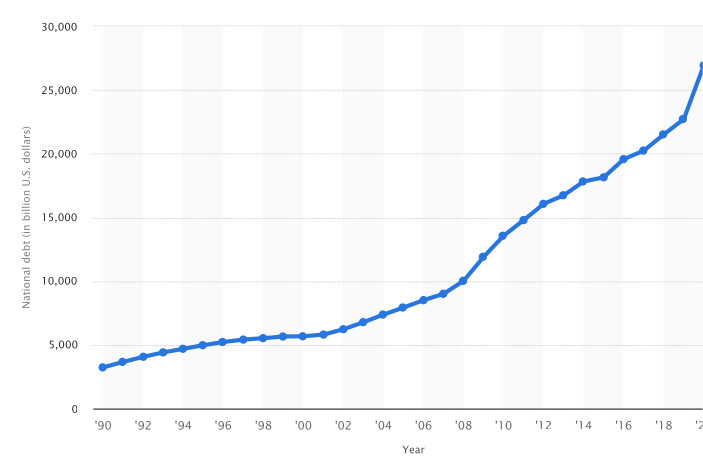
\includegraphics[width=\linewidth]{external/debt.jpg}
\end{image}%
\tcblower
\end{figureptx}%
\footnotetext[6]{US Department of the Treasury. (September 30, 2021). Public debt of the United States from 1990 to 2021 (in billion U.S. dollars) [Graph]. In Statista. Retrieved April 18, 2022, from \href{https://www.statista.com/statistics/187867/public-debt-of-the-united-states-since-1990/}{\nolinkurl{https://www.statista.com/statistics/187867/public-debt-of-the-united-states-since-1990/}}\label{g:fn:idp1847375496}}%
\par\medskip\noindent%
\textbf{National Debt.}\space\space%
\begin{exercisegroup}
\begin{divisionexerciseeg}{1}{}{1in}{x:exercise:national-debt-1}%
What is a simpler way to express 2000 billion dollars?\end{divisionexerciseeg}%
\begin{divisionexerciseeg}{2}{}{1in}{x:exercise:national-debt-2}%
Imagine a stack of 1,000 one‐dollar bills, which is about 4.3 inches tall. Imagine combining 1,000 stacks of 1,000 one‐dollar bills. How much money is in the stack?\end{divisionexerciseeg}%
\begin{divisionexerciseeg}{3}{}{1in}{x:exercise:national-debt-3}%
How tall would that stack be, in inches?  How tall in feet (rounded to the nearest foot)\end{divisionexerciseeg}%
\end{exercisegroup}
\par\medskip\noindent
\clearpage
\par\medskip\noindent%
\textbf{National Debt continued.}\space\space%
\begin{exercisegroup}
\begin{divisionexerciseeg}{4}{}{1in}{x:exercise:national-debt-4}%
Now imagine combining 1000 stacks like the one above in exercise \hyperlink{x:exercise:national-debt-2}{Worksheet Exercise~{\xreffont 1.2.2}}. How much money is in the stack?\end{divisionexerciseeg}%
\begin{divisionexerciseeg}{5}{}{1in}{x:exercise:national-debt-5}%
How tall would that stack be, in feet? How tall would that stack be, in miles? (Round to the nearest mile)\end{divisionexerciseeg}%
\begin{divisionexerciseeg}{6}{}{1in}{x:exercise:national-debt-6}%
Now imagine combining 1000 stacks like the one in exercise \hyperlink{x:exercise:national-debt-4}{Worksheet Exercise~{\xreffont 1.2.4}}. . How much money is in the stack?\end{divisionexerciseeg}%
\begin{divisionexerciseeg}{7}{}{1in}{x:exercise:national-debt-7}%
How tall would that stack be, in miles?\end{divisionexerciseeg}%
\end{exercisegroup}
\par\medskip\noindent
\clearpage
\par\medskip\noindent%
\textbf{Problem Situation 2:  Scientific Notation.}\space\space%
You saw that 1 billion can be written as 1,000,000,000 or represented as \(10^9\).  How would 2 billion be represented?  Since 2 billion is 2 times 1 billion, then 2 billion can be written as \(2 \times 10^9\).  Writing numbers in this way is called scientific notation.  Scientific notation is used primarily for writing very large numbers and very small numbers.  In this lesson, we will focus on large numbers.%
\par
The form for scientific notation is \(M \times 10^n\) where \(1\leq M < 10\).  The exponent equals the number of decimal places between the location of the decimal in the number as written in standard notation and the number written in scientific notation.%
\par
For example, if the number 500 were to be written in scientific notation, it could be thought of as \(5 \times 100\) or \(5 \times 10 \times 10\) which is equal to \(5 \times 10^2\).  The decimal point has been moved 2 places which corresponds to the exponent of 2.%
\par
Likewise, if the number 4300 were to be written in scientific  notation, it could be thought of as \(4.3 \times 1000\) or \(4.3 \times 10 \times 10 \times 10\) which is equal to \(4.3 \times 10^3\).  The decimal point has been moved 3 places (between 4300. and 4.3) which corresponds to the exponent of 3.%
\begin{exercisegroup}
\begin{divisionexerciseeg}{8}{}{}{x:exercise:scientific-notation-1}%
Write the numbers below in both standard notation and scientific notation. \begin{tableptx}{\textbf{}}{g:table:idp1847165576}{}%
\centering%
{\tabularfont%
\begin{tabular}{Blll}\hrulemedium
\multicolumn{1}{BlB}{Words}&\multicolumn{1}{lB}{Standard Notation}&\multicolumn{1}{lB}{Scientific Notation}\tabularnewline\hrulemedium
\multicolumn{1}{BlB}{four hundred}&\multicolumn{1}{lB}{\tablecelllines{l}{m}
{\(\hspace{2in}\)\\
\\
}
}&\multicolumn{1}{lB}{\tablecelllines{l}{m}
{\(\hspace{2in}\)\\
\\
}
}\tabularnewline\hrulemedium
\multicolumn{1}{BlB}{twenty three thousand}&\multicolumn{1}{lB}{\tablecelllines{l}{m}
{\\
\\
}
}&\multicolumn{1}{lB}{\tablecelllines{l}{m}
{\\
\\
}
}\tabularnewline\hrulemedium
\multicolumn{1}{BlB}{7.2 million}&\multicolumn{1}{lB}{\tablecelllines{l}{m}
{\\
\\
}
}&\multicolumn{1}{lB}{\tablecelllines{l}{m}
{\\
\\
}
}\tabularnewline\hrulemedium
\end{tabular}
}%
\end{tableptx}%
\end{divisionexerciseeg}%
\begin{divisionexerciseeg}{9}{}{}{x:exercise:scientific-notation-2}%
The table below contains the national deficit and national debt for various years.  Write the number in both standard notation and scientific notation. \begin{tableptx}{\textbf{}}{g:table:idp1847201160}{}%
\centering%
{\tabularfont%
\begin{tabular}{Blll}\hrulemedium
\multicolumn{1}{BlB}{Words}&\multicolumn{1}{lB}{Standard Notation}&\multicolumn{1}{lB}{Scientific Notation}\tabularnewline\hrulemedium
\multicolumn{1}{BlB}{1965 deficit:  \textdollar{}1.41 billion}&\multicolumn{1}{lB}{\tablecelllines{l}{m}
{\(\hspace{2in}\)\\
\\
}
}&\multicolumn{1}{lB}{\tablecelllines{l}{m}
{\(\hspace{2in}\)\\
\\
}
}\tabularnewline\hrulemedium
\multicolumn{1}{BlB}{2009 deficit:  \textdollar{}1412.69 billion}&\multicolumn{1}{lB}{\tablecelllines{l}{m}
{\\
\\
}
}&\multicolumn{1}{lB}{\tablecelllines{l}{m}
{\\
\\
}
}\tabularnewline\hrulemedium
\multicolumn{1}{BlB}{2014 deficit:  \textdollar{}484.6 billion}&\multicolumn{1}{lB}{\tablecelllines{l}{m}
{\\
\\
}
}&\multicolumn{1}{lB}{\tablecelllines{l}{m}
{\\
\\
}
}\tabularnewline\hrulemedium
\multicolumn{1}{BlB}{2014 debt:     \textdollar{}18.2 trillion}&\multicolumn{1}{lB}{\tablecelllines{l}{m}
{\\
\\
}
}&\multicolumn{1}{lB}{\tablecelllines{l}{m}
{\\
\\
}
}\tabularnewline\hrulemedium
\end{tabular}
}%
\end{tableptx}%
\end{divisionexerciseeg}%
\end{exercisegroup}
\par\medskip\noindent
\clearpage
\par\medskip\noindent%
\textbf{Problem Situation 3: Comparing the Sizes of Numbers.}\space\space%
One of the skills you will learn in this course is how to write quantitative information. A writing principle that you will use throughout the course is given below followed by Question 2, which gives you an example of how to use this principle.%
\par
Writing Principle: Use specific and complete information. The reader should understand what you are trying to say even if they have not read the question or writing prompt. This includes%
%
\begin{itemize}[label=\textbullet]
\item{}information about context, and%
\item{}quantitative information%
\end{itemize}
\begin{exercisegroup}
\begin{divisionexerciseeg}{10}{}{}{x:exercise:writing-principle-1}%
A \href{http://www.tallahassee.com/story/news/2014/06/03/scott-vetoes-million-billion-state-budget/9901117/}{headline in 2014}\footnotemark{} read “Scott vetoes \textdollar{}69 million in \textdollar{}77-billion state budget”.  Is the \textdollar{}69 million a small or large portion of the total state budget?  The following four statements are all correct. Which statement provides the best description, based on the writing principle? %
\begin{enumerate}[label=(\alph*)]
\item{}The portion vetoed is a very small part of the entire state budget%
\item{}\textdollar{}69 million is about a thousandth of \textdollar{}77 billion%
\item{}The \textdollar{}69 million vetoed is a very small part of the entire state budget of \textdollar{}77 billion%
\item{}The \textdollar{}69 million that was vetoed is about one tenth of one percent of the total \textdollar{}77 billion state budget.%
\end{enumerate}
\end{divisionexerciseeg}%
\footnotetext[7]{\nolinkurl{http://www.tallahassee.com/story/news/2014/06/03/scott-vetoes-million-billion-state-budget/9901117/}\label{g:fn:idp1847252232}}%
\begin{divisionexerciseeg}{11}{}{}{x:exercise:writing-principle-2}%
The federal budget in 2012 included \textdollar{}471 billion for Medicare and \textdollar{}47 billion for International Affairs.  Complete the statement below that compares the two quantities. \begin{quote}%
The budget of \textdollar{}471 billion for Medicare is about \fillin{2.272727272727273} times larger than the \textdollar{}47 billion budget for International Affairs.%
\end{quote}
\end{divisionexerciseeg}%
\begin{divisionexerciseeg}{12}{}{1in}{x:exercise:writing-principle-3}%
Using the writing principle above, in a full sentence compare the 2009 deficit and the 2014 deficit from exercise \hyperlink{x:exercise:scientific-notation-2}{Worksheet Exercise~{\xreffont 1.2.9}}\end{divisionexerciseeg}%
\end{exercisegroup}
\par\medskip\noindent
\clearpage
\par\medskip\noindent%
\textbf{Estimate.}\space\space%
For each situation below, describe your estimation strategy for each situation.  Include your final estimated quantity.  Then tell me if your quantity is in the millions, billions, trillions, or some other size, such as tens of millions.\begin{exercisegroup}
\begin{divisionexerciseeg}{13}{}{1in}{x:exercise:nation-wide-min-wage-increase}%
About 3 million working people in the U.S. make at or below the federal minimum wage of \textdollar{}7.25 per hour.  Estimate the amount of money needed per year to raise their wages to \textdollar{}15 per hour.\end{divisionexerciseeg}%
\begin{divisionexerciseeg}{14}{}{1in}{x:exercise:nation-wide-girl-scout-cookies}%
The amount of money needed to buy everyone in the United States a box of Girl Scout cookies.\end{divisionexerciseeg}%
\begin{divisionexerciseeg}{15}{}{1in}{x:exercise:state-wide-college}%
The amount of money needed to send all adults in your state to college for four years.\end{divisionexerciseeg}%
\begin{divisionexerciseeg}{16}{}{1in}{x:exercise:us-national-debt}%
If the U.S. national debt was \textdollar{}22 trillion in 2019, and was evenly divided among the people living in the United States, how much would each person's share be?\end{divisionexerciseeg}%
\end{exercisegroup}
\par\medskip\noindent
\par\medskip\noindent%
\textbf{Calculate.}\space\space%
Now use a calculator to refine your estimates from above.\begin{exercisegroup}
\begin{divisionexerciseeg}{17}{}{1in}{x:exercise:calculate-ation-wide-min-wage-increase}%
About 3 million working people in the U.S. make at or below the federal minimum wage of \textdollar{}7.25 per hour.  Estimate the amount of money needed per year to raise their wages to \textdollar{}15 per hour.\end{divisionexerciseeg}%
\begin{divisionexerciseeg}{18}{}{1in}{x:exercise:calc-nation-wide-girl-scout-cookies}%
The amount of money needed to buy everyone in the United States a box of Girl Scout cookies.\end{divisionexerciseeg}%
\end{exercisegroup}
\par\medskip\noindent
\clearpage
\par\medskip\noindent%
\textbf{Calculate (continued).}\space\space%
\begin{exercisegroup}
\begin{divisionexerciseeg}{19}{}{1in}{x:exercise:calc-state-wide-college}%
The amount of money needed to send all adults in your state to college for four years.\end{divisionexerciseeg}%
\begin{divisionexerciseeg}{20}{}{1in}{x:exercise:calc-us-national-debt}%
If the U.S. national debt was \textdollar{}22 trillion in 2019, and was evenly divided among the people living in the United States, how much would each person's share be?\end{divisionexerciseeg}%
\end{exercisegroup}
\par\medskip\noindent
\par\medskip\noindent%
\textbf{Percent of National Debt.}\space\space%
\begin{exercisegroup}
\begin{divisionexerciseeg}{21}{}{1in}{x:exercise:est-percent-debt}%
If the U.S. budget is about \textdollar{}4.1 trillion, estimate the percentage of the budget which would be needed to pay for your estimate in Question 5 above.\end{divisionexerciseeg}%
\begin{divisionexerciseeg}{22}{}{1in}{x:exercise:calc-precent-debt}%
If the U.S. budget is about \textdollar{}4.1 trillion, calculate the percentage of the budget which would be needed to pay for your estimate in Question 9 above.  Round to the nearest hundredth of a percent.\end{divisionexerciseeg}%
\end{exercisegroup}
\par\medskip\noindent
\clearpage
\par\medskip\noindent%
\textbf{Fast Food Restaurant Budget.}\space\space%
Let's say that your favorite fast food restaurant employees 20 minimum-wage workers who each work, on average, five hours in a day.  The daily overhead (electricity, food, etc.) is about \textdollar{}300 a day, and the daily revenue from sales is about \textdollar{}1,200 a day. \begin{tableptx}{\textbf{}}{g:table:idp1847289480}{}%
\centering%
{\tabularfont%
\begin{tabular}{Bllllllll}\hrulemedium
\multicolumn{1}{BlB}{}&\multicolumn{1}{lB}{A}&\multicolumn{1}{lB}{B}&\multicolumn{1}{lB}{C}&\multicolumn{1}{lB}{D}&\multicolumn{1}{lB}{E}&\multicolumn{1}{lB}{F}&\multicolumn{1}{lB}{G}\tabularnewline\hrulemedium
\multicolumn{1}{BlB}{1}&\multicolumn{1}{lB}{Employees\(\hspace{.25 in}\)}&\multicolumn{1}{lB}{Av. hours\(\hspace{.25 in}\)}&\multicolumn{1}{lB}{Wages (\textdollar{} per hour)}&\multicolumn{1}{lB}{Total Labor Cost}&\multicolumn{1}{lB}{Overhead\(\hspace{.75 in}\)}&\multicolumn{1}{lB}{Revenue\(\hspace{.75 in}\)}&\multicolumn{1}{lB}{Profit.\(\hspace{1 in}\)}\tabularnewline\hrulemedium
\multicolumn{1}{BlB}{2}&\multicolumn{1}{lB}{\tablecelllines{l}{m}
{\\
\\
\\
}
}&\multicolumn{1}{lB}{}&\multicolumn{1}{lB}{}&\multicolumn{1}{lB}{}&\multicolumn{1}{lB}{}&\multicolumn{1}{lB}{}&\multicolumn{1}{lB}{}\tabularnewline\hrulemedium
\end{tabular}
}%
\end{tableptx}%
\begin{exercisegroup}
\begin{divisionexerciseeg}{23}{}{}{x:exercise:fast-food-a}%
Fill in the four numbers above into the spreadsheet above, and also fill in the minimum wage.\end{divisionexerciseeg}%
\begin{divisionexerciseeg}{24}{}{1in}{x:exercise:fast-food-b}%
What spreadsheet formula should go in cell D2? (If nobody in your group has used spreadsheets before, flag down your instructor for help or search online.)\end{divisionexerciseeg}%
\begin{divisionexerciseeg}{25}{}{1in}{x:exercise:fast-food-c}%
What spreadsheet formula should go in cell G2?\end{divisionexerciseeg}%
\begin{divisionexerciseeg}{26}{}{1in}{x:exercise:fast-food-d}%
If we wanted to copy the numbers and formulas in row 2 into rows 3 and 4, how would we do it?\end{divisionexerciseeg}%
\begin{divisionexerciseeg}{27}{}{1in}{x:exercise:orders-of-mag-connections}%
Record the important mathematical ideas from the discussion.\end{divisionexerciseeg}%
\end{exercisegroup}
\par\medskip\noindent
\end{worksheet-subsection-numberless}
\restoregeometry
%
%
\typeout{************************************************}
\typeout{Exercises 1.2 Out of Class Exercises}
\typeout{************************************************}
%
\begin{exercises-subsection-numberless}{Out of Class Exercises}{}{Out of Class Exercises}{}{}{x:exercises:ex-orders-of-mag}
A website recommends that you should have at least 1 gallon of water for every inch of goldfish length in your tank.\footnote{Retrieved from https:\slash{}\slash{}www.cuteness.com\slash{}article\slash{}many-can-fit-gallon-tank, accessed January 25, 2019.\label{g:fn:idp1847361416}}%
\begin{divisionexercise}{1}{}{}{x:exercise:three-billion-goldfish}%
If you have 3 billion goldfish that are each 3 inches long, how many gallons of water would you need?\end{divisionexercise}%
\begin{divisionexercise}{2}{}{}{x:exercise:georgia-aquarium}%
The \href{https://www.georgiaaquarium.org/}{Georgia Aquarium}\footnotemark{} broke the record for the world's largest aquarium in 2005 with a tank that holds 6.3 million gallons of water.  How many of these record-breaking tanks would it take to house the 3 billion goldfish that are each three inches long?\end{divisionexercise}%
\footnotetext[9]{\nolinkurl{georgiaaquarium.org}\label{g:fn:idp1847356936}}%
\begin{divisionexercise}{3}{}{}{x:exercise:sun-burn-out}%
Scientists predict that the sun will burn out in about five billion years.  How many minutes is that?\end{divisionexercise}%
\begin{divisionexercise}{4}{}{}{x:exercise:gracie-building-a}%
Gracie wishes to buy a commercial building to expand her business and needs to save for the downpayment.  If she can save \textdollar{}4,000 a month, \emph{estimate} (i.e. do not use a calculator) how long it will take to save \textdollar{}2,000,000 if does not earn interest on her savings.  Assume (unrealistically) that the price of the building won't change while she saves.\end{divisionexercise}%
\begin{divisionexercise}{5}{}{}{x:exercise:gracie-building-b}%
Explain your thought process for your estimate to the answer above.\end{divisionexercise}%
\begin{divisionexercise}{6}{}{}{x:exercise:gracie-building-c}%
Calculate how long it will take.\end{divisionexercise}%
\begin{divisionexercise}{7}{}{}{x:exercise:gracie-building-d}%
Do you think this is a reasonable amount of time? Explain.\end{divisionexercise}%
\begin{divisionexercise}{8}{}{}{x:exercise:gracie-building-e}%
Estimate how much she would need to save each month to realize her goal in 15 years.\end{divisionexercise}%
\begin{divisionexercise}{9}{}{}{x:exercise:gracie-building-f}%
Explain how you came up with your estimate.\end{divisionexercise}%
\begin{divisionexercise}{10}{}{}{x:exercise:gracie-building-g}%
Now calculate how much she would need to save each month to realize her goal in 15 years.  Round to the nearest cent.\end{divisionexercise}%
The main hall of Grand Central Station in New York City is approximately \textdollar{}210,000\textdollar{} square feet.%
\begin{divisionexercise}{11}{}{}{x:exercise:grand-central-a}%
Estimate how many people could stand with enough room to turn around in the main hall of the station if there were an emergency which required that the station be used to shelter people.\end{divisionexercise}%
\begin{divisionexercise}{12}{}{}{x:exercise:grand-central-b}%
Explain how you came up with your estimate.\end{divisionexercise}%
\begin{divisionexercise}{13}{}{}{x:exercise:grand-central-c}%
If there are 4 million people in Manhattan, NY, on a typical workday, estimate the percentage of them that could be sheltered in the station.\end{divisionexercise}%
\begin{divisionexercise}{14}{}{}{x:exercise:grand-central-d}%
Explain how you came up with your estimate.\end{divisionexercise}%
\end{exercises-subsection-numberless}
\end{sectionptx}
\end{chapterptx}
%
%
\typeout{************************************************}
\typeout{Chapter 2 (No title)}
\typeout{************************************************}
%
\begin{chapterptx}{(No title)}{}{(No title)}{}{}{x:chapter:ch-empty}
\begin{introduction}{}%
Try adding your own content here!%
\end{introduction}%
\end{chapterptx}
%
%
\typeout{************************************************}
\typeout{Chapter 3 Examples of PreTeXt features}
\typeout{************************************************}
%
\begin{chapterptx}{Examples of PreTeXt features}{}{Examples of PreTeXt features}{}{}{x:chapter:ch_pretext-features}
\begin{introduction}{}%
Below are examples of a lot of PreTeXt elements.%
\end{introduction}%
%
%
\typeout{************************************************}
\typeout{Section 3.1 Environments and Blocks}
\typeout{************************************************}
%
\begin{sectionptx}{Environments and Blocks}{}{Environments and Blocks}{}{}{x:section:sec_ptxfeat-blocks}
Some text%
\begin{theorem}{My Theorem.}{}{x:theorem:thm-my-theorem}%
Theorem statement.%
\end{theorem}
\begin{proof}{}{g:proof:idp1860801016}
Proof of theorem.%
\end{proof}
\begin{example}{}{g:example:idp1860804216}%
Statement of example%
\par\smallskip%
\noindent\textbf{\blocktitlefont Solution}.\hypertarget{g:solution:idp1860806904}{}\quad{}The solution.%
\end{example}
Now a figure. (Uncomment the source to include Tikz, SagePlot, and Asymptote examples built with \mono{pretext build -d}.)%
\begin{figureptx}{A frog}{g:figure:idp1860813432}{}%
\begin{image}{0.25}{0.5}{0.25}%
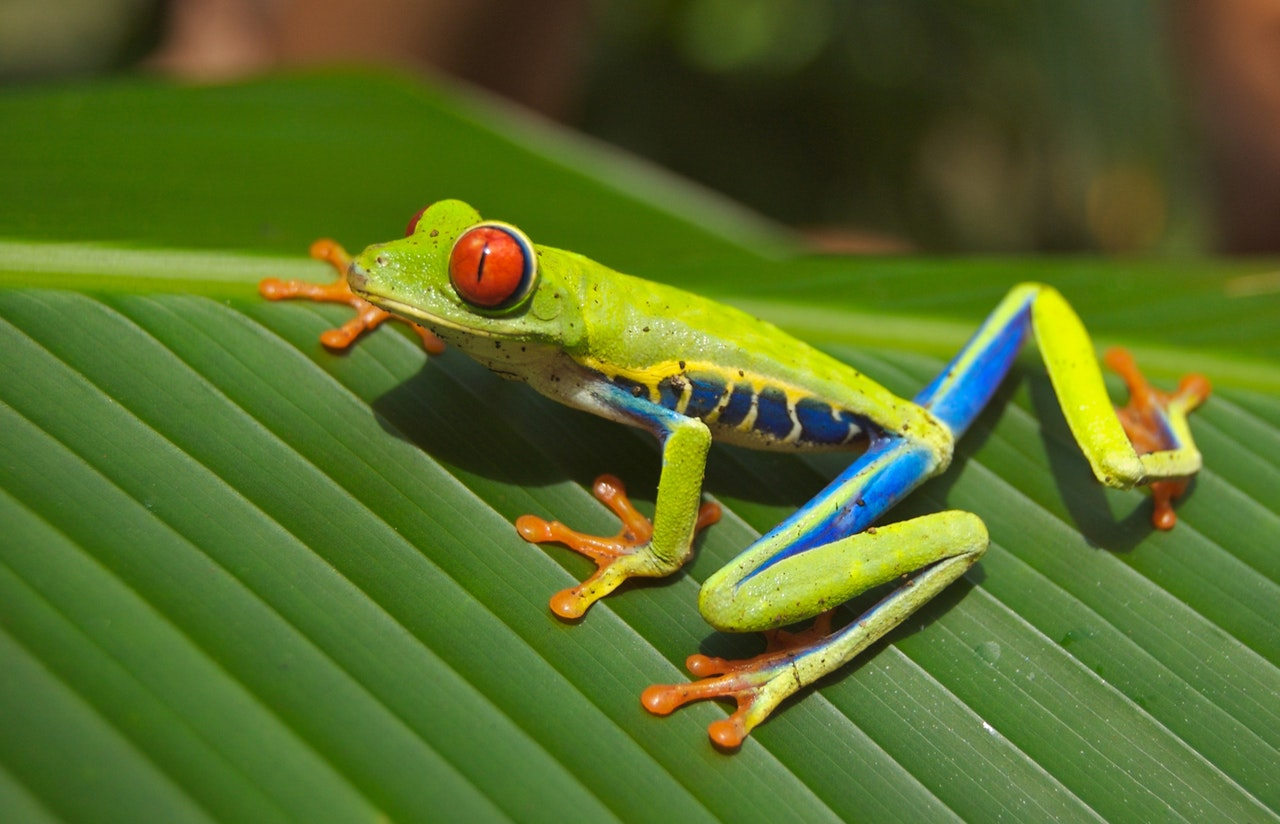
\includegraphics[width=\linewidth]{external/frog.jpg}
\end{image}%
\tcblower
\end{figureptx}%
\begin{figureptx}{The graph \(C_5\) made by TikZ}{x:figure:figure-tikz-example-diagram}{}%
\begin{image}{0.4}{0.2}{0.4}%
\resizebox{\linewidth}{!}{%
\begin{tikzpicture}
\coordinate (A) at (90+360/5:1);
\coordinate (B) at (90+2*360/5:1);
\coordinate (C) at (90+3*360/5:1);
\coordinate (D) at (90+4*360/5:1);
\coordinate (E) at (90:1);

\draw (A) -- (B) -- (C) -- (D) -- (E) -- (A);
\foreach \x in {(A), (B), (C), (D), (E)}{
    \fill \x circle (2pt);
}
\end{tikzpicture}
}%
\end{image}%
\tcblower
\end{figureptx}%
\begin{figureptx}{Canada}{x:figure:figure-asy-example-diagram}{}%
\begin{image}{0}{1}{0}%

\includegraphics[width=\linewidth]{generated/asymptote/cflag.pdf}
\end{image}%
\tcblower
\end{figureptx}%
\end{sectionptx}
%
%
\typeout{************************************************}
\typeout{Section 3.2 Another section}
\typeout{************************************************}
%
\begin{sectionptx}{Another section}{}{Another section}{}{}{x:section:section-2-2}
This will have more stuff%
\end{sectionptx}
\end{chapterptx}
%
\appendix%
%
\clearpage\phantomsection%
\addcontentsline{toc}{part}{Appendices}%
%
%
\typeout{************************************************}
\typeout{Appendix A Selected Hints}
\typeout{************************************************}
%
\begin{solutions-chapter}{Selected Hints}{}{Selected Hints}{}{}{g:solutions:idp1860823672}
\end{solutions-chapter}
%
%
\typeout{************************************************}
\typeout{Appendix B Selected Solutions}
\typeout{************************************************}
%
\begin{solutions-chapter}{Selected Solutions}{}{Selected Solutions}{}{}{g:solutions:idp1860827768}
\end{solutions-chapter}
%
%
\typeout{************************************************}
\typeout{Appendix C List of Symbols}
\typeout{************************************************}
%
\begin{appendixptx}{List of Symbols}{}{List of Symbols}{}{}{g:appendix:idp1860831224}
\begin{longtable}[l]{lp{0.60\textwidth}r}
\addtocounter{table}{-1}
\textbf{Symbol}&\textbf{Description}&\textbf{Page}\\[1em]
\endfirsthead
\textbf{Symbol}&\textbf{Description}&\textbf{Page}\\[1em]
\endhead
\multicolumn{3}{r}{(Continued on next page)}\\
\endfoot
\endlastfoot
\end{longtable}
\end{appendixptx}
%
\backmatter%
%
\clearpage\phantomsection%
\addcontentsline{toc}{part}{Back Matter}%
%
%% The index is here, setup is all in preamble
%% Index locators are cross-references, so same font here
{\xreffont\printindex}
%
\cleardoublepage
\pagestyle{empty}
\vspace*{\stretch{1}}
\begin{backcolophon}{g:colophon:idp1860828536}%
This book was authored in PreTeXt.%
\end{backcolophon}%
\vspace*{\stretch{2}}
\end{document}